%%%%%%%%%%%%%%%%%%%%%%%%%%%%%%%%%%%%%%%
%  Modèle LaTeX pour les documents TB
%
%  Par Charles Duchêne, IG JI
%  Juin 2013
%
%  Toutes les images doivent se trouver
%  dans un sous-dossier pictures
%
%%%%%%%%%%%%%%%%%%%%%%%%%%%%%%%%%%%%%%%

\documentclass[12pt,a4paper]{article}
\RequirePackage[utf8]{inputenc} 
\RequirePackage[T1]{fontenc}
\usepackage[english,francais]{babel}
\usepackage[pdftex]{hyperref}	
\usepackage[Rennes,version]{telecom}	
\usepackage{aeguill}
\usepackage{times}
\usepackage{listingsutf8}
\usepackage{makeidx}
\usepackage{glossaries}
\makeindex
\makeglossary

%%%%%%%%%%%%%%%%%%%%%%%%%%%%
% Variables pour ce document
%%%%%%%%%%%%%%%%%%%%%%%%%%%%
\author{Charles \textsc{Duchêne}, élève ingénieur\\\url{charles.duchene@telecom-bretagne.eu}}			% service émetteur ou auteur
\title{Modèle \LaTeX{} Télécom Bretagne}									% titre du document
\contributors{}													% contributeurs
\version{1.0}													% version du document, avec option version
\docdescription{Documentation utilisateur : comment utiliser le modèle \LaTeX{} pour Télécom Bretagne ?}	% description en première de couverture
%%%%%%%%%%%%%%%%%%%%%%%%%%%
%%% FICHIER DE CONFIGURATION OPTIONNEL

%%%%%%%% Propriétés pdf %%%%%%%%%%%
\hypersetup{
	bookmarks=true,
	unicode= yes,
	pdftitle={Document témoin du modèle LaTeX pour Télécom Bretagne},
	pdfauthor={Charles Duchêne},
	pdfsubject={},
	pdfkeywords={Télécom, TB, modèle, LaTeX},
	colorlinks=true,
	linkcolor=black,
	citecolor=black,
	filecolor=black,
	urlcolor = black
}

\lstset{
	basicstyle=\ttfamily\small,
	breaklines=true,
	keywordstyle=\bfseries\color{TBbrun},
	inputencoding=utf8/latin1,
}

\lstdefinestyle{stylelatex}{%
	language=tex,
	morekeywords={usepackage,newcommand,begin,renewcommand,section,
	TBannexe,TBsommaire,subsection},
	commentstyle=\itshape\color{TBvert}
}

\lstnewenvironment{latex}{%
	\lstset{style=stylelatex}}{}

\lstnewenvironment{bash}{%
\lstset{
	language=bash,
	basicstyle=\color{white}\ttfamily\small,
	keywordstyle=\color{TBvert}\bfseries,
	backgroundcolor=\color{black},
	morekeywords={sudo, cp, mkdir},
	deletekeywords={local},
}
}{}
 % fichier de configuration optionnel


%%%% DÉBUT DOCUMENT
\begin{document}
% ne pas modifier ! imprime la première page du document
\TBfrontcover

%% Affichage des listes et tables.
\TBsommaire
%\listoffigures  % décommenter pour avoir la liste des figures
%\listoftables   % décommenter pour avoir la liste des tables

%%%%%%%%%%%%%%%%%%%%%%%%%%%%
%     CORPS DU DOCUMENT
%%%%%%%%%%%%%%%%%%%%%%%%%%%%
\section{Présentation}
\subsection{Adaptation du modèle Microsoft Word -- OpenOffice}
\subsubsection{Première de couverture}
La première de couverture comprend :
\begin{itemize}
	\item le nom de l'auteur ou du service émetteur ;
	\item la date (date de compilation\footnote{Commande \texttt{today} utilisée.}) ;
	\item éventuellement les noms des contributeurs ;
	\item la frise, non flottante (positionnée à 9 cm du côté gauche et à 17 cm du bas de page) ;
	\item le titre, espacé de 2 cm de la frise et de 2 cm du texte suivant ;
	\item éventuellement un numéro de version (cf. \ref{optionversion}) ;
	\item éventuellement une description du document, alignée à gauche, non justifiée, dans une case de 7 cm ;
	\item le logo avec la mention Institut Mines-Télécom, non flottant (positioné à 9 cm du côté gauche et à 2 cm du bas de page).
\end{itemize}\bigskip

Le texte est aligné à gauche à 9 cm du côté gauche. La marge entre le haut de page et le nom de l'auteur (premier texte) est de 7,5 cm.  L'interligne est de 1,5. Le texte est en fonte normale, taille par défaut\footnote{Pour ce document 12 pt, comme pour le modèle Word.}, excepté le titre qui est en gras et \og large \fg\footnote{Ce qui correspond pour un corps de texte de 12 pt à 14 pt, comme pour le modèle Word.}.

\subsubsection{Corps du texte}

Le corps du texte est en taille de police définie au début du document. Le retrait simple correspond à un alinéa typographique de taille 2,5 ex. Les marges sont de 2 cm en haut et en bas et de 3 cm à gauche et à droite.\\ 
Le titre de premier niveau (\texttt{section}) est entiérement en majuscule, de couleur noir, en gras et en 16 pt. Un point (\og . \fg) est ajouté après le numéro.\\
Le titre de deuxième niveau (\texttt{subsection}) est en petites capitales, de couleur vert\footnote{Vert \og Télécom \og accessible par \texttt{TBvert} avec (R,G,B)=(168,181,10)}, en gras et en 14 pt. Ils sont espacés de la marge de gauche d'une indentation.\\
Le titre de troisième niveau (\texttt{subsubsection}) est de couleur brun \footnote{Brun \og Télécom \og accessible par \texttt{TBbrun} avec (R,G,B)=(109,80,71)}, en gras. Ils sont espacés de la marge de gauche de deux indentations.\\
Le titre de quatrième niveau (\texttt{paragraph}) est de couleur noir, en gras et italique mais \textbf{non souligné}\footnote{Le soulignement des titres est mal géré en \LaTeX{} et ne correspond pas à une bonne pratique en typographie française. \emph{Petites leçons de typographies}, Jacques \textsc{André}, p. 23, nov. 2012, éditions du Jobet.}. Ils ne sont pas espacés de la marge de gauche.\\
Les pages sont numérotées en chiffres arabes, le numéro de page est centré en bas de page.\\

\begin{itemize}
	\item les puces de premier niveau sont des carrés pleins ;
		\begin{itemize}
			\item celles de second niveau sont des tirets.
		\end{itemize}
\end{itemize}\bigskip

Le retrait de second niveau n'est pas supporté mais peut éventuellement être obtenu de manière \og barbare \fg\footnote{En l'occurence \texttt{\textbackslash hspace*\{5ex\}}.}.\\

\noindent Concernant le sommaire : 
\begin{itemize}
	\item le nom du sommaire est centré et écrit en vert, en bas de casse ;
	\item seuls les titres de niveau supérieur au égal à 3 sont affichés ;
	\item les titres de premier niveau sont en majuscules, en gras et 14 pt ;
	\item les titres de deuxième niveau sont en petites majuscules, en gras ;
	\item les titres de troisième niveau sont en fonte normale.
\end{itemize}
À noter qu'il n'y a pas d'indentation par niveau.\\

\noindent Enfin, concernant les annexes (voir \ref{annexe} pour l'utilisation de la commande) :
\begin{itemize}
	\item le titre des annexes est écrit en brun et est centré ;
	\item le numéro n'apparaît pas ;
	\item dans le sommaire, le numéro apparaît après le titre de l'annexe ;
	\item les sections et inférieures n'apparaissent pas dans le sommaire ;
	\item les sections des annexes sont numérotées par lettres  majuscules ;
	\item la numérotation des sections est remise à \og A \fg{} à chaque nouvelle annexe.
\end{itemize}\bigskip

\subsubsection{Dernière de couverture}

La dernière de couverture comprend :
\begin{itemize}
	\item l'adresse du campus\footnote{Possibilité est laissée de choisir le campus, voir \ref{optioncampus}.}, située à 20 cm du haut de page et à 9 cm du côté gauche, écrit en 10 pt ;
	\item le logo de l'École seul, non flottant (positioné à 2,7 cm du bas et 9 cm du côté gauche).
\end{itemize}

\subsubsection{Différences avec le modèle officiel}

Malgré toute l'attention apportée, il reste des différences entre ce modèle \LaTeX{} et le modèle officiel prévu pour Microsoft Word ou OpenOffice :
\begin{itemize}
	\item le double retrait n'est pas géré ;
	\item les titres de quatrième niveau ne sont pas soulignés ;
	\item le numéro de page n'apparaît pas sur la dernière de couverture ;
	\item la police de la chartre n'est pas nativement supportée par \LaTeX\footnote{Il est cependant possible d'utiliser ladite police en utilisant les \texttt{.tff}.}{} ;
	\item certaines tailles de police ou espacements diffèrent.
\end{itemize} \bigskip

\emph{Note aux lecteurs : n'hésitez pas à signaler toute autre différence à \url{charles.duchene@telecom-bretagne.eu} !}

\subsection{Installer le modèle}

Il n'est pas nécessaire d'installer le modèle, cependant, cela oblige à copier le fichier \texttt{telecom.sty} ainsi que les logos à chaque fois qu'un nouveau document doit être créé, ce qui n'est absolument pas optimal. Cette section indique comment procéder.

\subsubsection{Distribution \TeX Live (Linux et Mac)}

Voici les commandes nécessaires à l'installation du modèle sur votre machine (procédure pour Linux, adaptation pour Mac laissée à l'initiative du lecteur) : 

\begin{bash}
operateur@machine:$ cd /usr/local/share/texmf/tex/latex/
operateur@machine:$ sudo mkdir telecom
operateur@machine:$ cd telecom
operateur@machine:$ sudo cp ~/Downloads/modele_telecom/telecom.sty . 
operateur@machine:$ sudo mkdir pictures
operateur@machine:$ sudo cp ~/Downloads/modele_telecom/pictures/* pictures/ 
operateur@machine:$ cd /usr/local/share/texmf/
operateur@machine:$ sudo mktexlsr
\end{bash}

Le modèle est désormais installé !

\subsubsection{Distribution MiK\TeX{} (Windows)}

Créer tout d'abord un dossier pour les paquets locaux\footnote{Il n'est pas recommandé d'utiliser le dépôt global de MiK\TeX.}, par exemple le dossier \texttt{C:\textbackslash Users\textbackslash you\textbackslash texmf}. Il s'agit ensuite de respecter l'architecture d'un dépôt \TeX. Créer pour cela l'arborescence suivante :\\
{\ttfamily
	C:\textbackslash Users\textbackslash you\textbackslash texmf \\
	\hspace*{0.5cm} tex \\
	\hspace*{1 cm} latex \\
	\hspace*{1.5 cm} telecom : y copier telecom.sty\\
	\hspace*{2 cm} pictures : y copier logo*, frise.png
}\\

\noindent Utiliser ensuite l'interface de MiK\TeX{} nommée \og Settings (admin) \fg.\\
Aller sur l'onglet \og Roots \fg{} et ajouter le dossier précédent : \texttt{C:\textbackslash Users\textbackslash you\textbackslash texmf}.\\
Aller sur l'onglet \og General \fg{} et cliquer sur \og Refresh FNDB \fg.\\

Le modèle est désormais installé !

\subsection{Utiliser le modèle}

Une fois le \textit{package} installé, il suffit de l'inclure pour profiter des commandes et du style définis pour Télécom Bretagne.
\begin{latex}
\usepackage{telecom}
\end{latex}

Les images doivent toutes se trouver dans un dossier nommé \texttt{pictures} ! \\
Il est recommandé de séparer les grandes parties du document en divers fichiers \texttt{.tex} et de les inclure. Pour ce document, toutes les parties ont été placées dans le dossier \texttt{includes}.

\subsubsection{Dépendances}

Les \textit{packages} suivants sont requis :
\begin{itemize}
\item appendix ;
\item setspace ;
\item eso-pic ;
\item xcolor ; 
\item graphicx ;
\item geometry ; 
\item titlesec ;
\item titletoc ;
\item MnSymbol.
\end{itemize}

\subsubsection{Utilisation des commandes}

\paragraph{Première de couverture}

La première de couverture est imprimée à l'aide de la commande \verb!\maketitle! redéfinie pour correspondre à la chartre. Elle utilise certaines macros \TeX{} et d'autres spécialement définies :
\begin{itemize}
	\item \texttt{author} pour l'auteur ou le service émetteur ;
	\item \texttt{title} ;
	\item \texttt{contributors} pour les éventuels contributeurs ;
	\item \texttt{docdescription} pour une éventuelle description du document, imprimée sur la première page ;
	\item \texttt{version}, à utiliser avec l'option \texttt{version} (cf. \ref{optionversion}).
\end{itemize}\bigskip

Pour rester cohérent avec le nom des autres commandes permettant d'obtenir un document aux couleurs de l'École, un alias, \verb!\TBfrontpage!, est également défini et amène au même résultat.

\paragraph{Sommaire}

La commande \verb!\TBsommaire! permet d'afficher le sommaire\footnote{Pour rappel, deux compilations sont nécessaires pour obtenir une table des matières à jour.}. Attention, il ne s'agit pas d'un alias sur la commande \verb!\tableofcontents! !

\paragraph{Annexes}
\label{annexe}

Pour commencer une nouvelle annexe : 
\begin{latex}
	\appendix % uniquemenent une fois
	
	\TBannexe{Titre de l'annexe} % rend Annexe 1 -- Titre de l'annexe
	\section{Section 1} % rend A Section 1
		\subsection{Subsection 1} % rend A.1 Subsection 1
	
	\TBannexe{Titre de la seconde annexe} % rend Annexe 2 -- Titre de la seconde annexe
	\section{Section 1} % rend A Section 1
\end{latex}

\paragraph{Index}

La commande \verb!\TBindex! permet d'afficher un index. Pour cela, il faut rajouter dans le préambule :
\begin{latex}
	\usepackage{makeidx}
	\makeindex
\end{latex}
et compiler avec \texttt{makeindex document.idx}. \\

Cette commande affiche l'index, écrit \og Index \fg{} en brun en haut de page de manière centrée et ajoute une ligne \og INDEX \fg{} au sommaire. Il ne s'agit pas que d'un alias sur la commande \verb!\printindex! !\\

Il est possible de modifier le nom de l'index avec cette commande :
\begin{latex}
	\renewcommand{\TBindexname}{Mon index}
\end{latex}

\paragraph{Bibliographie}

La commande \verb!\TBbiblio{style}{base}! permet d'afficher une bibliographie avec le style \texttt{style} en utilisant les ouvrages cités dans le fichier \texttt{base}. Cela écrit \og Références \fg{} en brun en haut de page de manière centrée et ajoute une ligne \og RÉFÉRENCES \fg{} au sommaire.\\

Il est possible de modifier le nom de la bibliographie avec cette commande :
\begin{latex}
	\renewcommand{\TBbiblioname}{Bibliographie}
\end{latex} \bigskip

Exemple d'utilisation :
\begin{latex}
	\TBbiblio{plain-fr}{includes/biblio}
\end{latex}

\paragraph{Glossaire}

La commande \verb!\TBglossary! permet d'afficher un glossaire. Pour cela, il faut rajouter dans le préambule :
\begin{latex}
	\usepackage[style...]{glossaries}
	\makeglossaries
\end{latex}
et compiler avec \texttt{makeindex -s document.ist -t document.tex.glg -o\\ document.gls document.glo}.\\

Cette commande affiche le glossaire, écrit \og Glossaire \fg{} en brun en haut de page de manière centrée et ajoute une ligne \og GLOSSAIRE \fg{} au sommaire. Il ne s'agit pas que d'un alias sur la commande \verb!\printglossary! !\\

Il est possible de modifier le nom du glossaire avec cette commande :
\begin{latex}
	\renewcommand{\TBglossaryname}{Mon glossaire}
\end{latex}

\paragraph{Dernière de couverture}

La dernière de couverture est affichée à l'aide de la commande \verb!\TBcoverpage!. Cette commande imprime le logo de l'École et l'adresse. En fonction du campus choisi (cf. \ref{optioncampus}), l'adresse est modifiée.

\section{Options disponibles}
\subsection{Afficher la version}
\label{optionversion}

Par défaut, le numéro de version n'est pas affiché sur la première de couverture, comme sur le modèle Word. Cependant, cette information peut être intéressante et une option du \textit{package} permet de le faire. \\

Pour cela, il suffit de préciser l'option \texttt{version} et d'instancier la macro correspondante.

\begin{latex}
\usepackage[version]{telecom}
[...]
\version{1.2.3}
[...]
\begin{document}
\end{latex}

\subsection{Choix du campus}
\label{optioncampus}

Sur la dernière de couverture est affichée l'adresse. Par défaut, il s'agit de l'adresse du campus de Brest, cependant, les options \texttt{Rennes} et \texttt{Toulouse} permettent d'afficher l'adresse du campus correspondant. \\
Noter que l'option \texttt{Brest} existe mais est optionnelle.\\

\begin{minipage}[c]{0.6\textwidth}
\begin{latex}
\usepackage{telecom}
% ou \usepackage[Brest]{telecom}
\end{latex}
\end{minipage}
\vrule\begin{minipage}[c]{0.4\textwidth}
\centering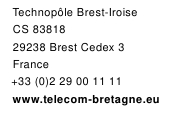
\includegraphics{brest}
\end{minipage}\\

\begin{minipage}[c]{0.6\textwidth}
\begin{latex}
\usepackage[Rennes]{telecom}
\end{latex}
\end{minipage}
\vrule\begin{minipage}[c]{0.4\textwidth}
\centering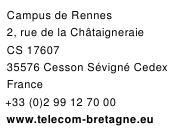
\includegraphics{rennes}
\end{minipage}\\

\begin{minipage}[c]{0.6\textwidth}
\begin{latex}
\usepackage[Toulouse]{telecom}
\end{latex}
\end{minipage}
\vrule\begin{minipage}[c]{0.4\textwidth}
\centering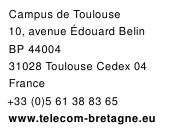
\includegraphics{toulouse}
\end{minipage}\\


% ANNEXES
\appendix
\TBannexe{Fichier telecom.sty}
\lstinputlisting[style=stylelatex]{telecom.sty}

% INDEX, RÉFÉRENCES et GLOSSAIRE
% \TBindex
% \TBbiblio{plain-fr}{includes/biblio}
% \TBglossary

% ne pas modifier ! imprime la dernière page du document
\TBcoverpage
\end{document}
